\chapter{Specific requirements}


\section{Functions}
To specify the functional requirements, that are all the fundamental actions that must take place in the we system we are proposing, along with the textual descriptions we provide some scenarios, sequence diagrams and use case diagrams, because we believe that they can be a valid support to our words.


\subsection{Taxi Request}\label{subsec:taxiRequest}


\paragraph{Scenario 1}{\small\itshape Alexei, Anna's husband, is out of town for work. Thus, she decides to go and visit her lover, Count Vronsky. She recently came to know that a new taxi service was active in the city, so after a brief lookup in the Internet she finds the website, myTaxiWeb.it. She finds out that there is an app as well, but she is too eager to meet her lover to download it, so she quickly fills in the form with her data (name and surname, mobile phone number, and her origin and destination addresses) to request a taxi ride. Her request is sent by the system to the nearest taxi driver, who is named Kostya and drives the taxi number T1878, and he accepts without hesitation by clicking the proper button on his company smartphone. In a few seconds Anna receives an SMS confirmation that taxi T1878 is due in four minutes. Then she puts some lipstick, grabs her handbag and calmly leaves. Kostya is already waiting for her in the street, and in twenty minutes or so she is hugging her beloved. As soon as she gets off his taxi, Kostia confirms that he is available again to the system, by clicking the proper icon on his smartphone.}


\paragraph{Scenario 2}{\small\itshape Jay is quite a wealthy man, and as it happens, he has not always lived a perfect life. Today, like every other month, he has an appointment with a man of his past, some Meyer, in a rough area of the town. So he opens myTaxiApp on his smartphone, to which he registered recently, and looks for his destination in the small set of saved addresses. Once he found it, he lets the GPS locate him, then confirms the request for a taxi ride. myTaxiService system looks for a driver in Jay's area, but there is none; fortunately, in an adjacent one there is George, on Taxi T1925, who has been idle for some time. However, as George sees the destination of the request, he immediately understands that he had better not go there, so he rejects the request. myTaxiService registers his refusal, but since the nearest taxi is about half an hour far from Jay, it asks him whether he wants to withdraw his reservation, which he does. He cannot be late at his appointment.}


\begin{figure*}
	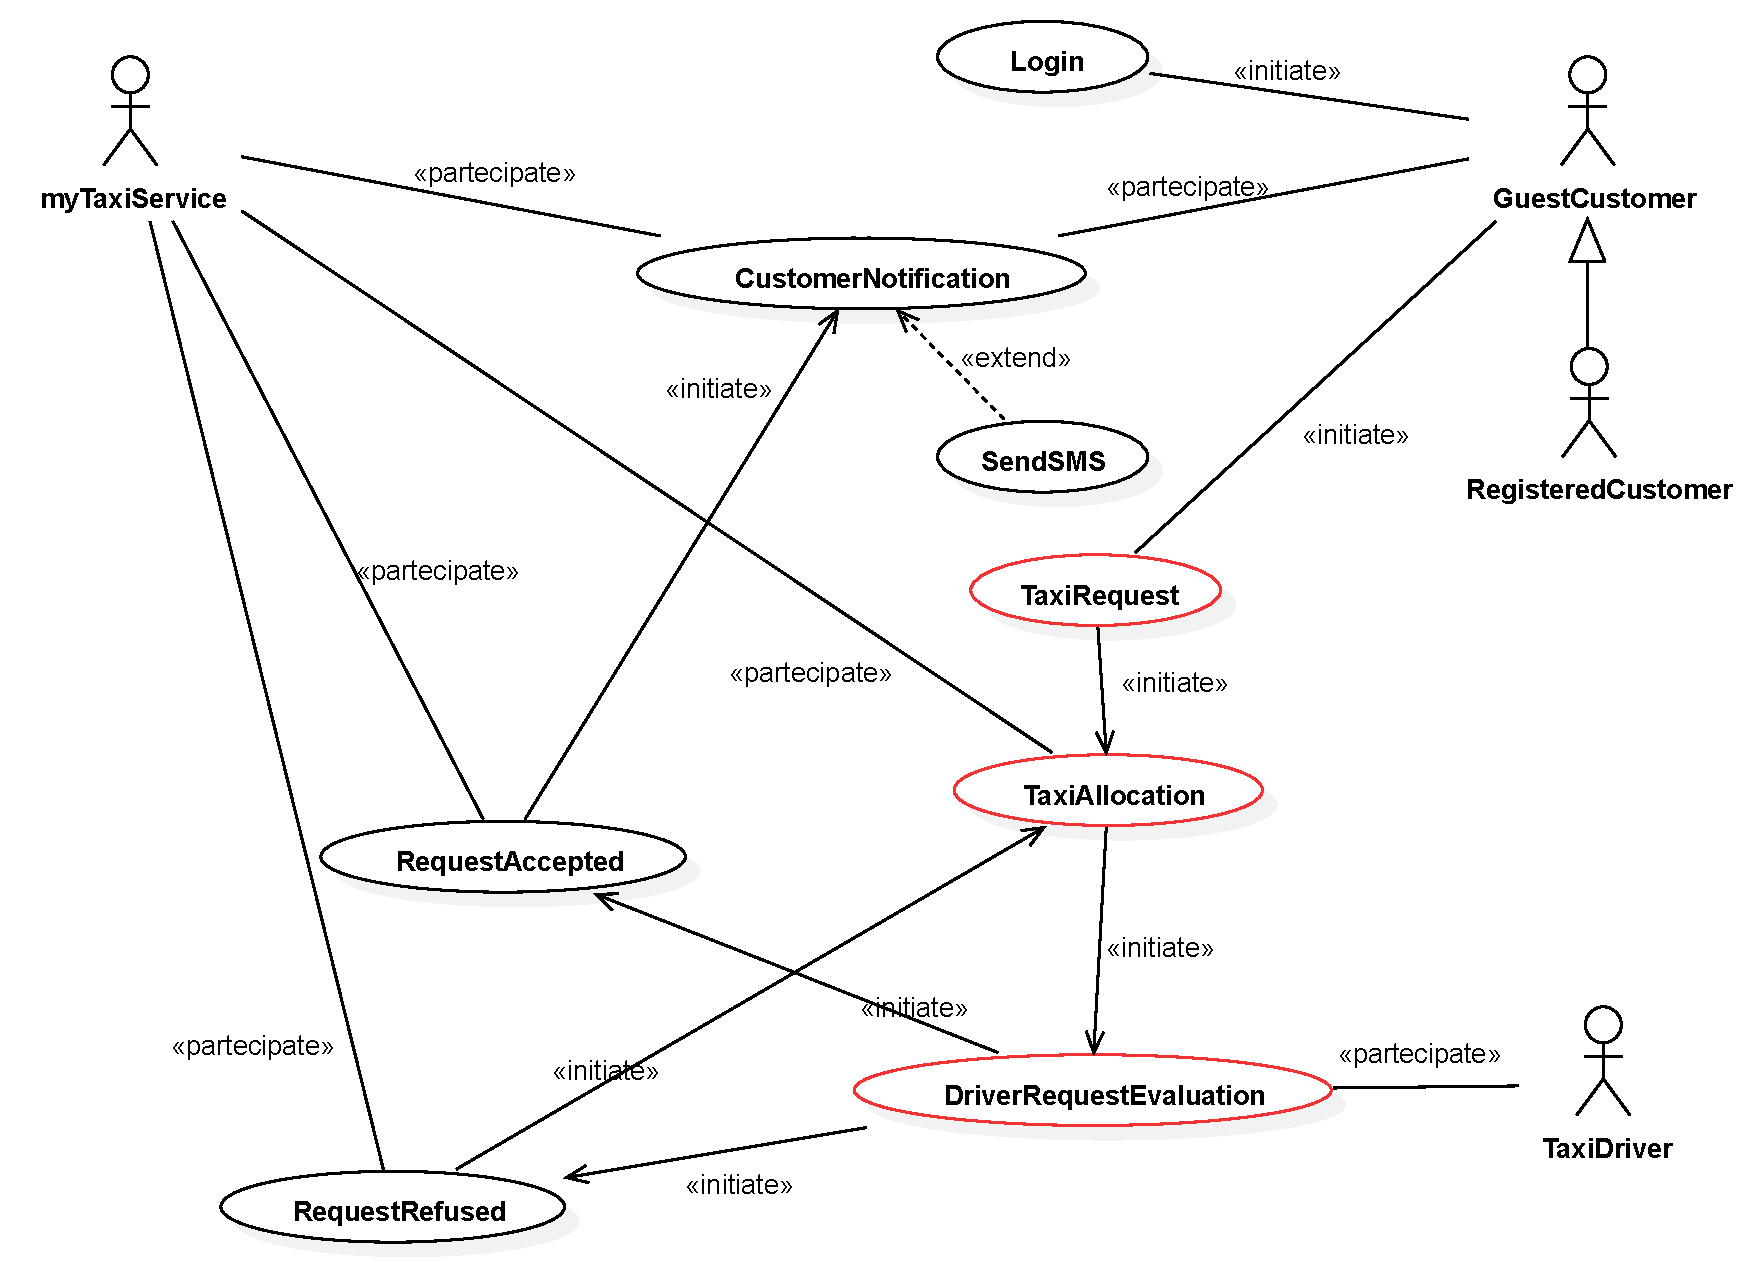
\includegraphics[width=\linewidth]{img/U_TaxiRequestGLOBAL}
	\caption{Comprehensive use case diagram for the taxi request. It will be further expanded in the following with more detailed diagrams.}
\end{figure*}	


\begin{figure*}
	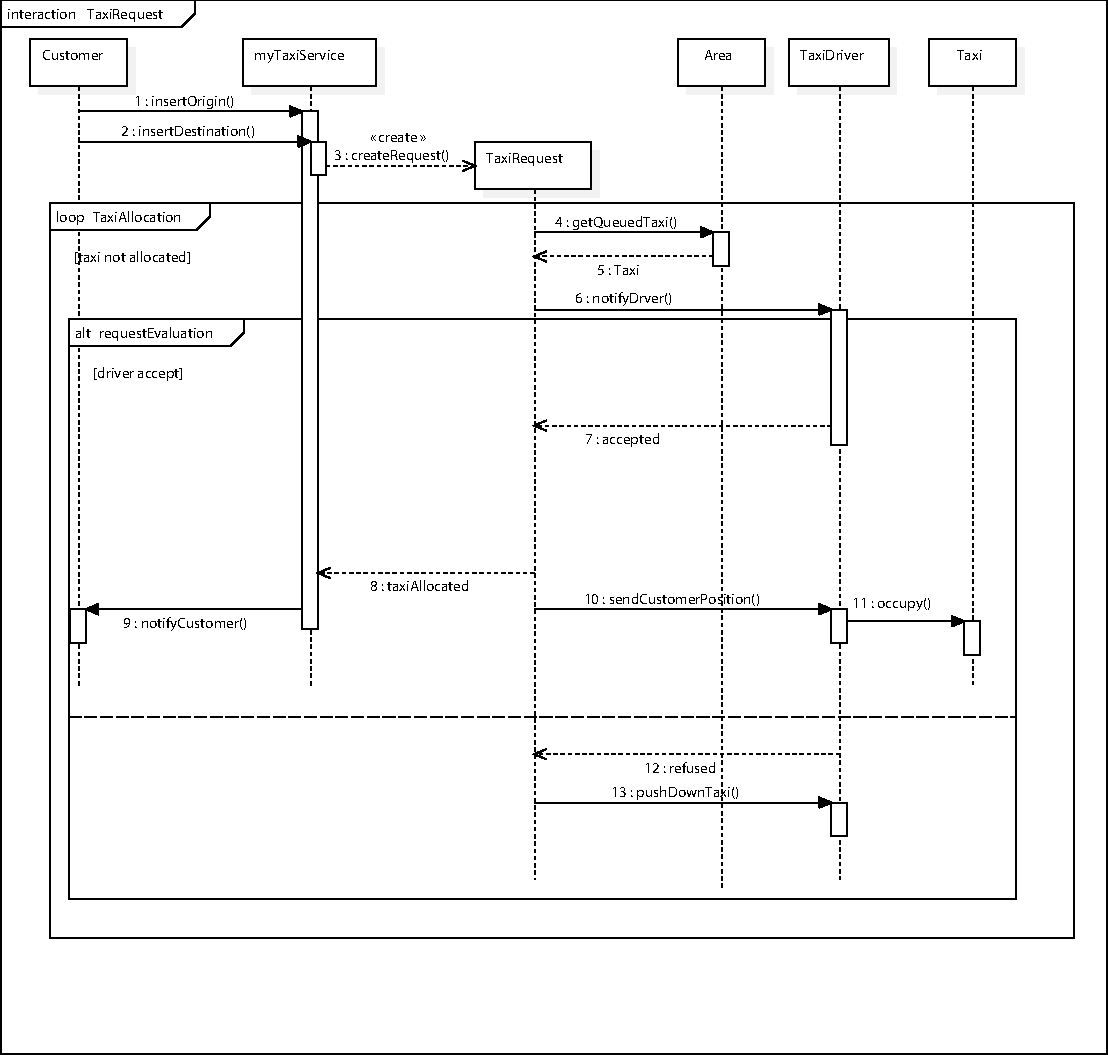
\includegraphics[width=\linewidth]{img/S_TaxiRequest}
	\caption{Sequence diagram for the taxi request analysis.}
\end{figure*}


\begin{tabularx}{\fullwidthlength}{ l X }
	\toprule
	name				&	TaxiRequest
	\\ \midrule
	actors				&	GuestCustomer, RegisteredCustomer
	\\ \midrule
	entry conditions	&	a customer opens myTaxiApp/myTaxiWeb to request a taxi
	\\ \midrule
	flow of events		&	\begin{enumerate}
	
		\item RegisteredCustomer can log in, GuestCustomer can sign in;
		
		\item GuestCustomer inserts his personal data, RegisteredCustomer views his personal data;
		
		\item GuestCustomer sends his GPS position or inserts the address, RegisteredCustomer can also select an address from the set of saved ones;
		
		\item Customer sends the request.
	
	\end{enumerate} \\ \midrule
	exit conditions		&	 all provided data are correct
	\\ \midrule
	exceptions			&	\begin{itemize}
		
		\item invalid address: an error message is shown and a correct addressed is requested
	
	\end{itemize} \\ \bottomrule
\end{tabularx}


\begin{figure}
	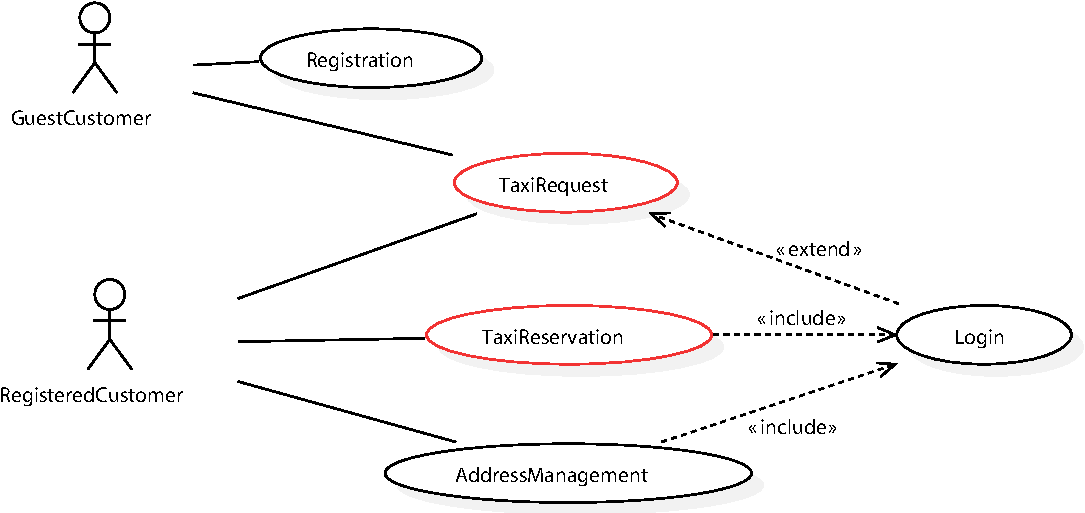
\includegraphics[width=\linewidth]{img/U_CustomerManagementGLOBAL}
	\caption{The customer can be either registered or guest. A guest can register and request a taxi (see figure \protect\ref{fig:taxiRequest}). A registered customer can make a reservation (see figure \protect\ref{subsec:taxiReservation}) and manage his favourite addresses.}
\end{figure}	


\begin{figure}
	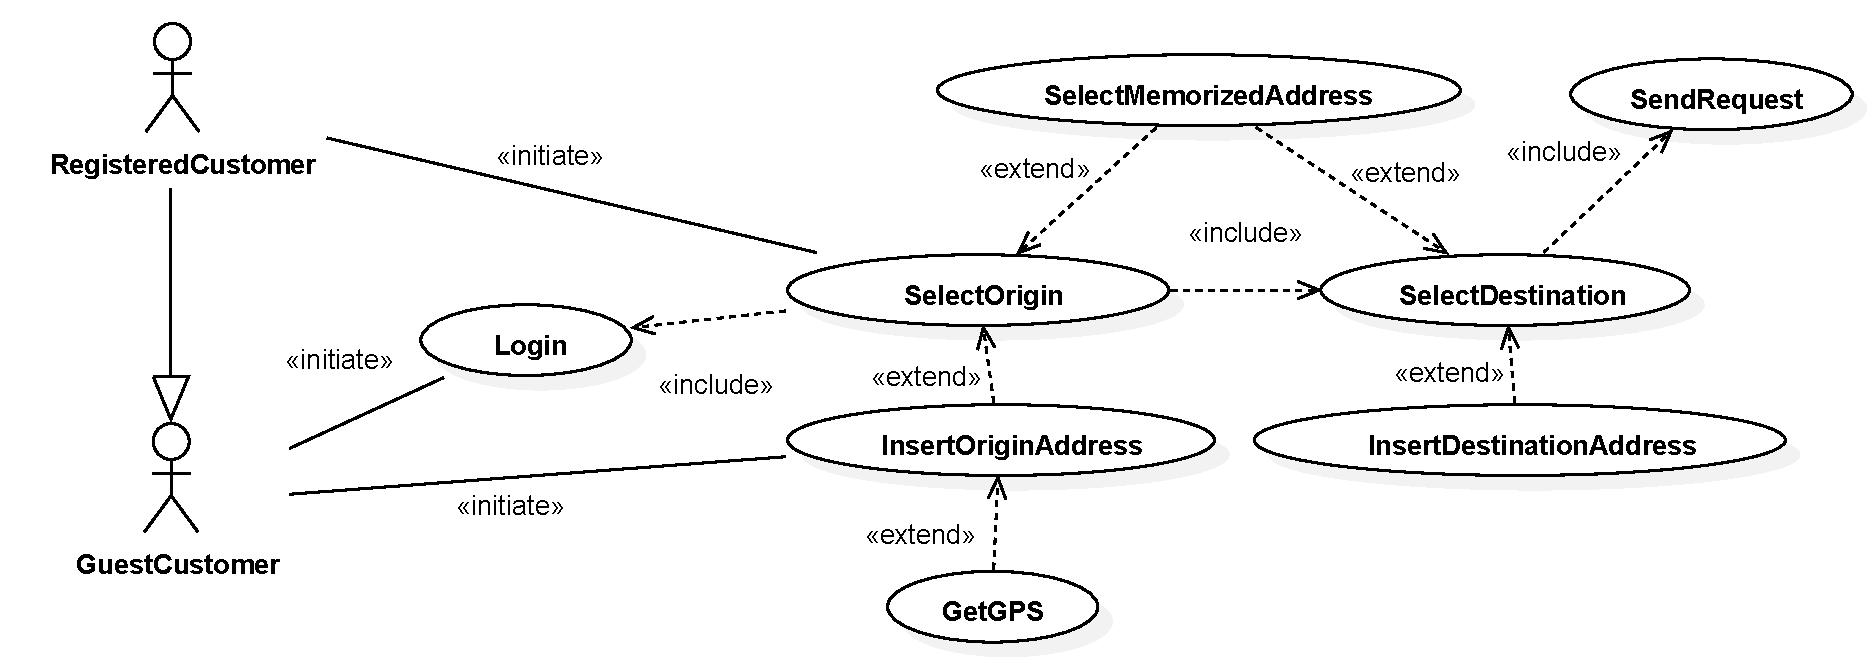
\includegraphics[width=\linewidth]{img/U_TaxiRequest.pdf}
	\caption{Detailed use case for the taxi ride request.}
	\label{fig:taxiRequest}	
\end{figure}	

%TODO rifare grafico (?)

\begin{tabularx}{\fullwidthlength}{ l X }
	\toprule
	name				&	TaxiAllocation
	\\ \midrule
	actors				&	myTaxiService
	\\ \midrule
	entry conditions	&	request received
	\\ \midrule
	flow of events		&	\begin{enumerate}
	
		\item the system determines the pertinence area;
	
		\item a request is sent to the first taxi driver in the taxi queue;
		
		\item if accepted, the address is sent to the driver, and the customer is notified with the time of arrival; otherwise the system proceeds to allocate the next taxi in the queue.
	
	\end{enumerate} \\ \midrule
	exit conditions		&	 driver has accepted the request
	\\ \midrule
	exceptions			&	\begin{itemize}
		
		\item if no taxis are available in the area, the system would recursively allocate the first taxi in the longest queue of the adjacent areas;
		
		\item if no taxis are available at all, the system notifies the customer of the situation and sends an estimated waiting time. The customer can cancel the request.
	
	\end{itemize} \\ \bottomrule
\end{tabularx}


\begin{figure}
	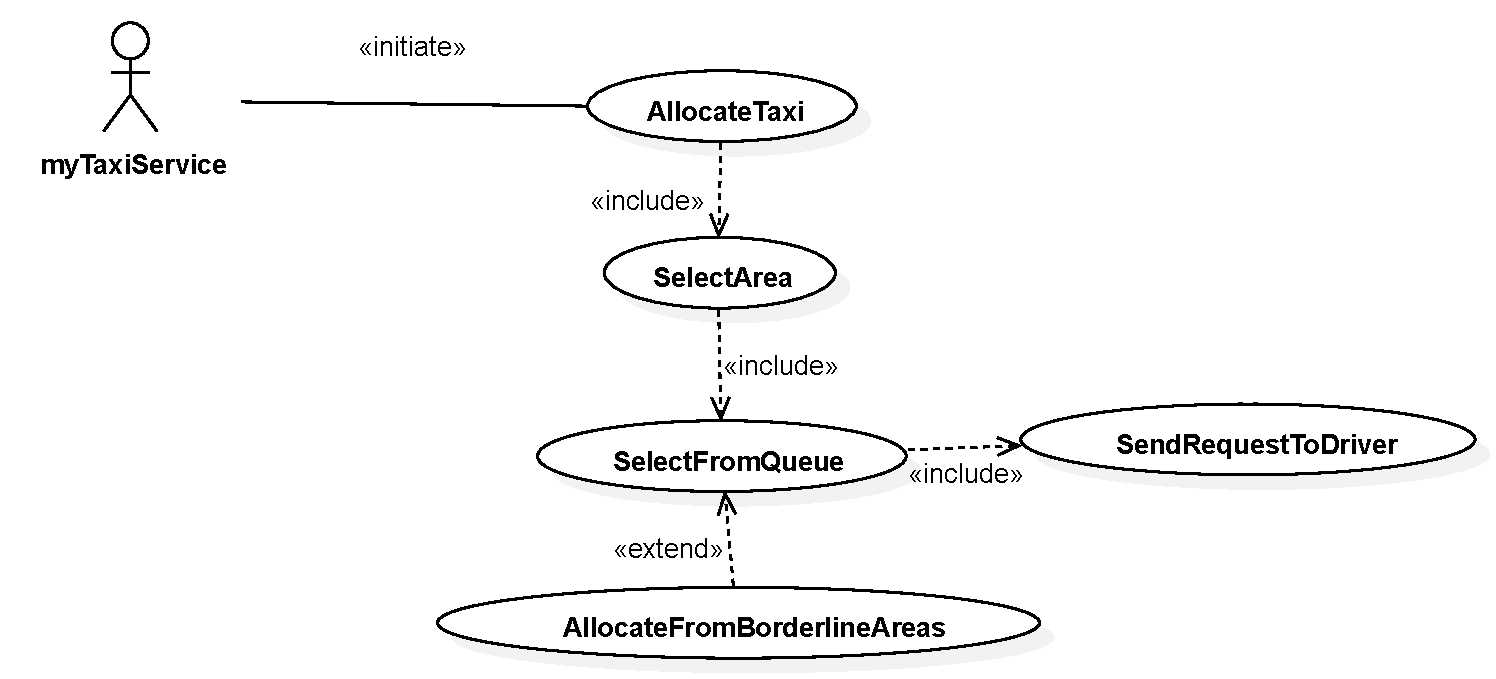
\includegraphics[width=\linewidth]{img/U_TaxiAllocation}
	\caption{Taxi allocation, from the point of view of myTaxiService.}
\end{figure}


\begin{figure}
	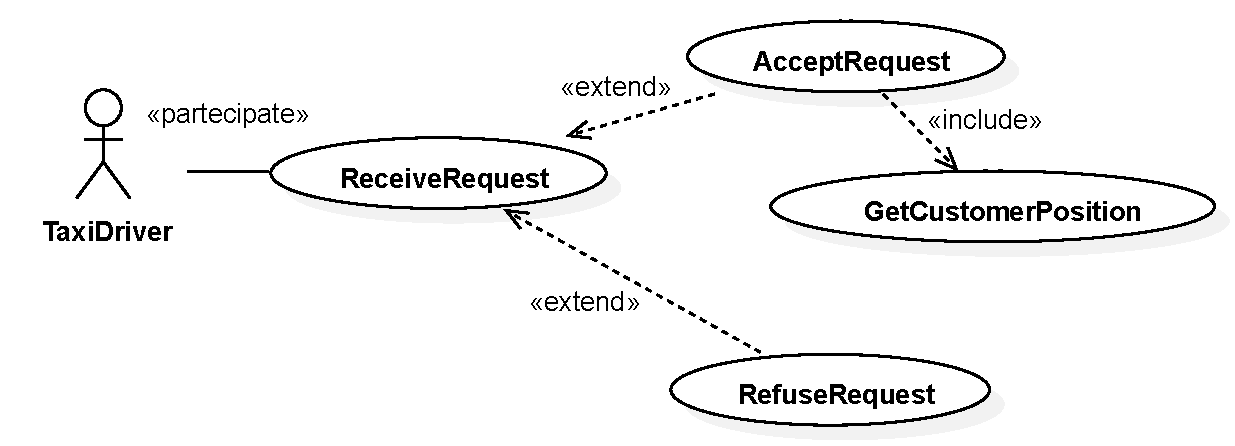
\includegraphics[width=\linewidth]{img/U_DriverRequestEvaluation.pdf}
	\caption{Taxi allocation, from the point of view of the taxi driver: he can either accept or reject the request.}
\end{figure}


%\newpage %forces the next subsection to only follow and not wrap the figure.
\begin{figure}[!h]
	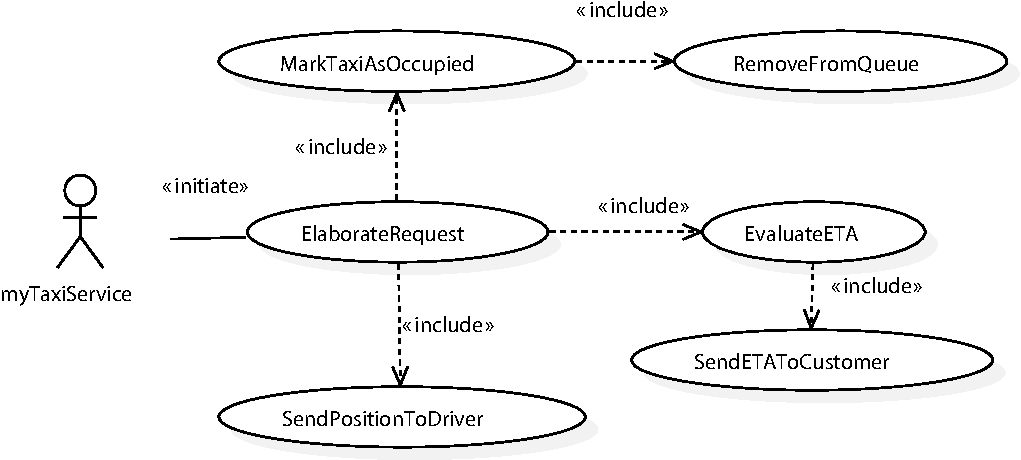
\includegraphics[width=\linewidth]{img/U_RequestAccepted}
	\caption{Request accepted use case, initiated by the acceptance of the request by the taxi driver.}
\end{figure}	


\begin{figure}
	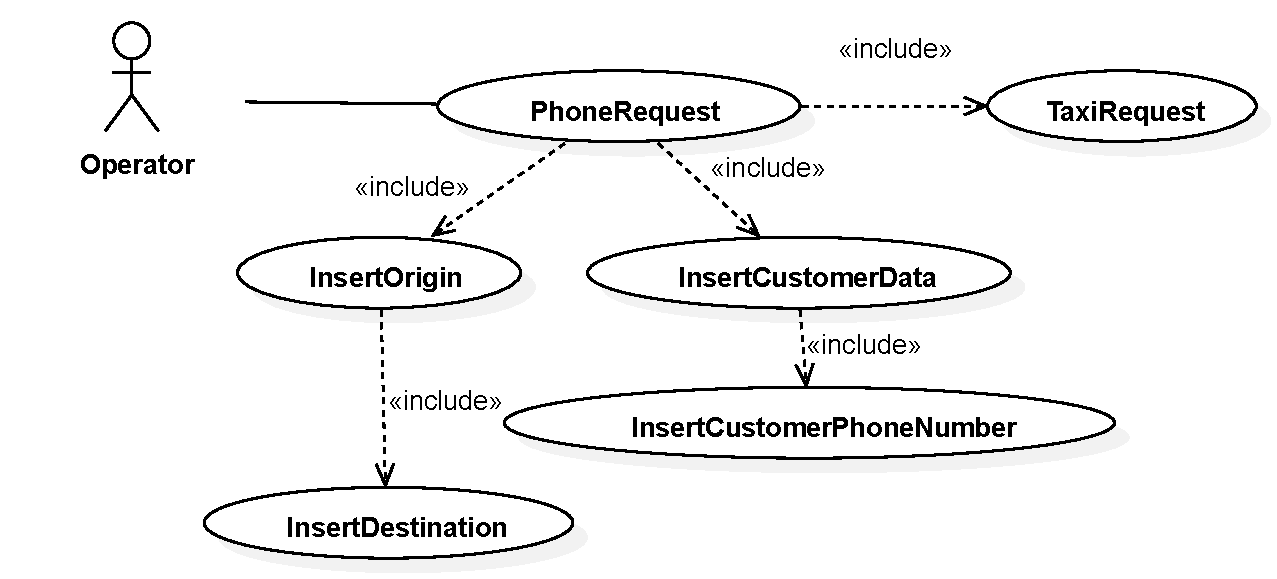
\includegraphics[width=\linewidth]{img/U_PhoneRequest}
	\caption{A customer may make a phone request. This is the relating use case diagram.}
\end{figure}	


\subsection{Taxi reservation}\label{subsec:taxiReservation}


\paragraph{Scenario}{\small\itshape Cookie has been in prison for a year, now. Her husband Lucious, notwithstanding the great weight of running a newly born entertainment company, growing three children all alone, and some sense of guilt for not being able to help her, wants their children to visit her. So tomorrow afternoon he is going to the jail by taxi with them. This morning, at about 9:30 AM, he tried to reserve a taxi, to guarantee a ride for themselves. However, his reservation was rejected, because he was making it more than \num{24} hours before the ride. But now, at 5:45PM, he tries again, and he is successful: his reservation is registered, and Lucious is notified that \num{10} minutes before the ride, he will receive a confirmation, with the number of the taxi too.}


\begin{figure*}
	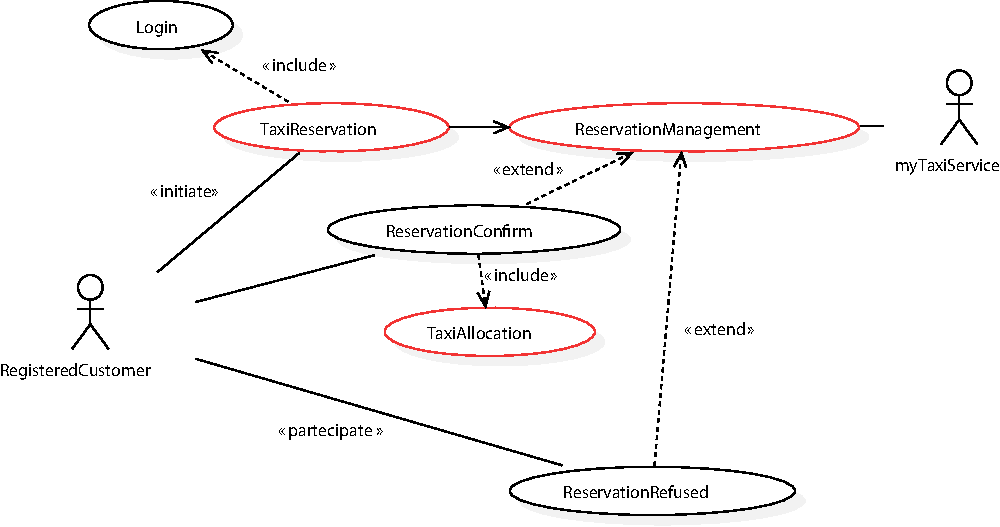
\includegraphics[width=\linewidth]{img/U_TaxiReservationGLOBAL}
	\caption{Comprehensive use case diagram for the taxi reservation. It will be further expanded in the following with more detailed diagrams.}
\end{figure*}


\begin{figure*}
	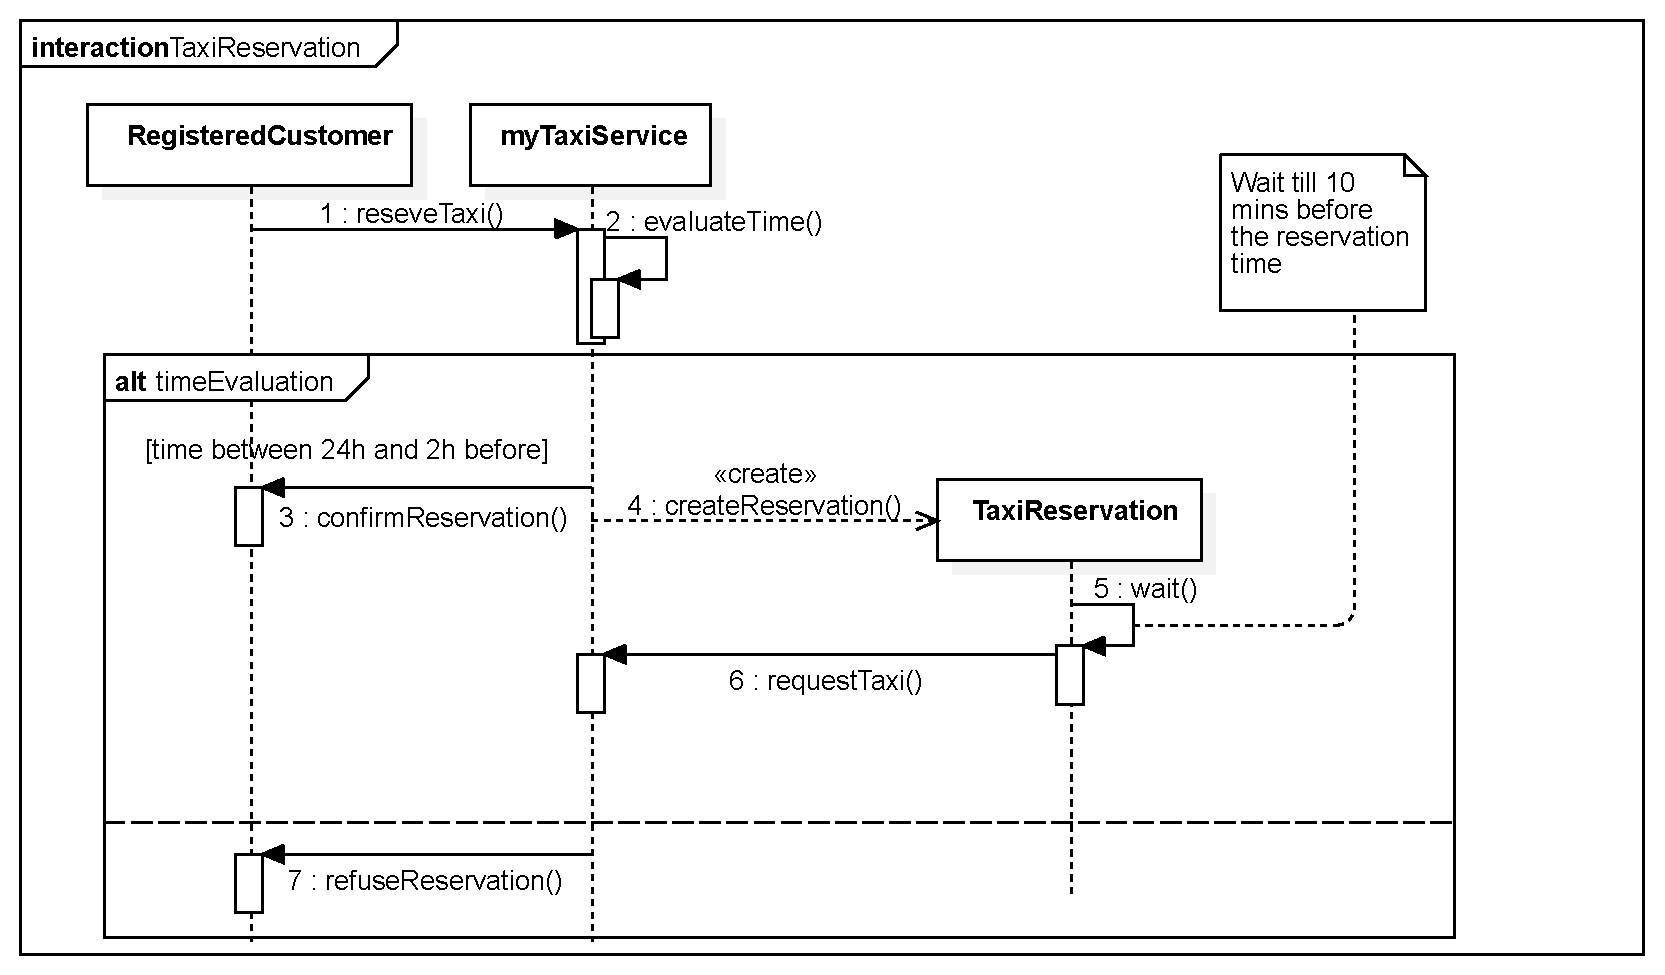
\includegraphics[width=\linewidth]{img/S_TaxiReservation}
	\caption{Sequence diagram for the taxi reservation analysis.}
\end{figure*}	


\begin{tabularx}{\fullwidthlength}{ l X }
	\toprule
	name				&	TaxiReservation
	\\ \midrule
	actors				&	RegisteredCustomer
	\\ \midrule
	entry conditions	&	RegisteredCustomer has successfully logged in
	\\ \midrule
	flow of events		&	\begin{enumerate}
	
		\item RegisteredCustomer inserts the origin address, select it from the favourite list or send his GPS position;
		
		\item RegisteredCustomer insert the destination address or select it from the favourite list;

		\item RegisteredCustomer selects the time;
		
		\item The reservation is sent
	
	\end{enumerate} \\ \midrule
	exit conditions		&	no exit condition
	\\ \midrule
	exceptions			&	\begin{itemize}
		
		\item invalid address: an error message is shown and a correct addressed is requested
	
	\end{itemize} \\ \bottomrule
\end{tabularx}



\begin{figure}
	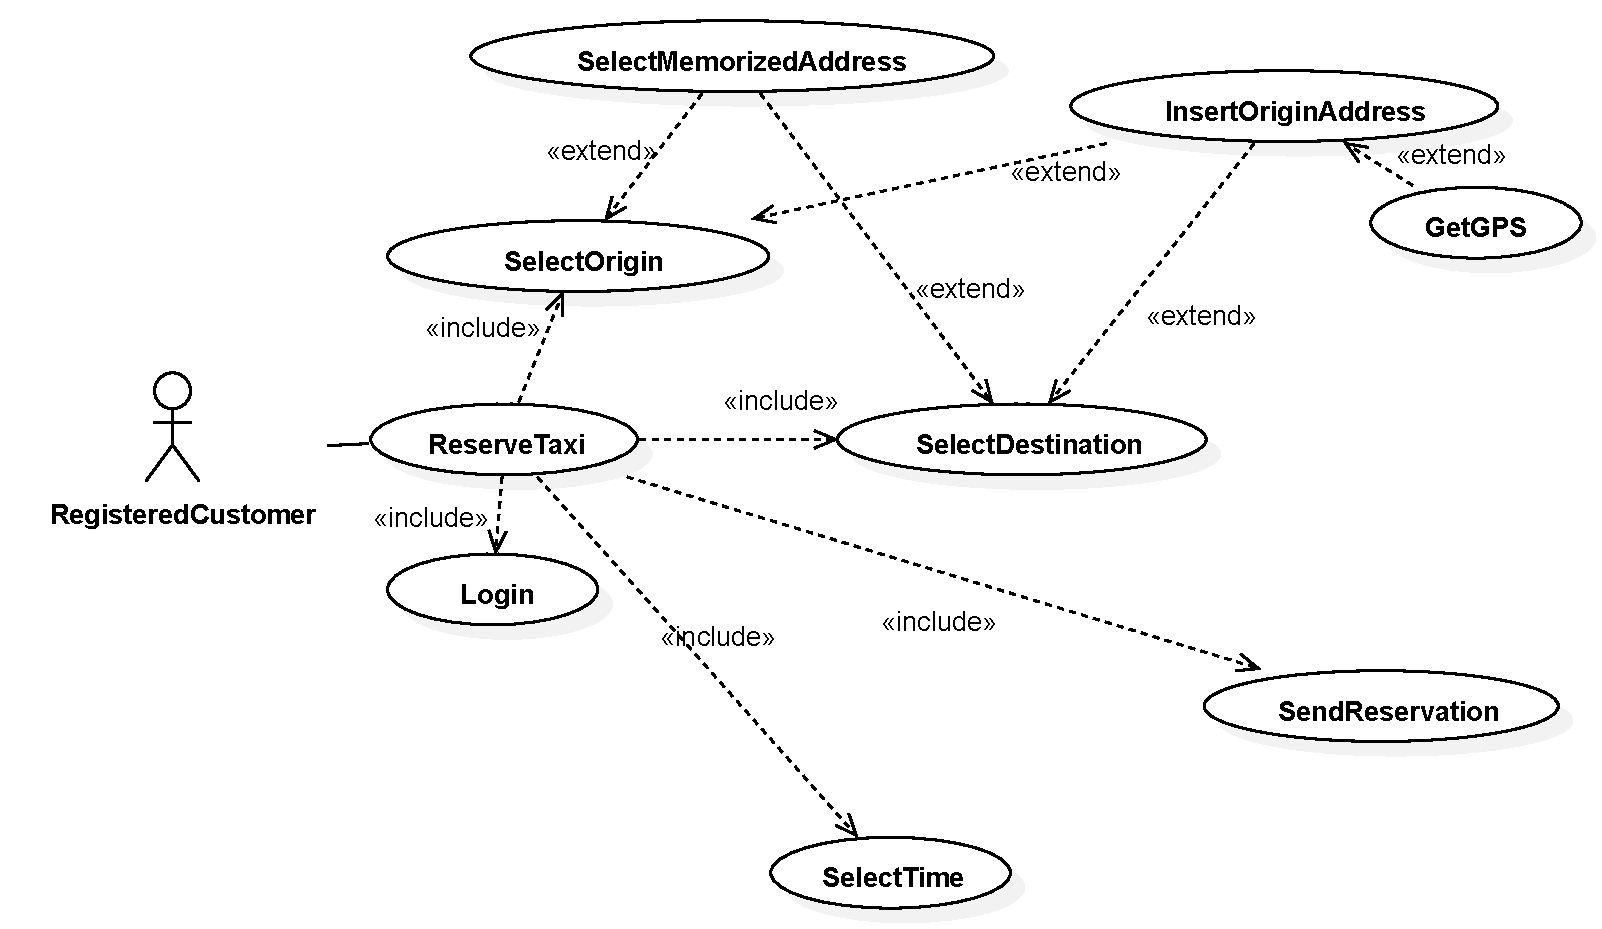
\includegraphics[width=\linewidth]{img/U_TaxiReservation}
	\caption{Detailed use case for the taxi ride reservation, from the point of view of the customer.}
\end{figure}


\begin{tabularx}{\fullwidthlength}{ l X }
	\toprule
	name				&	ReservationManagement
	\\ \midrule
	actors				&	myTaxiService
	\\ \midrule
	entry conditions	&	reservation received
	\\ \midrule
	flow of events		&	\begin{enumerate}
	
		\item the system evaluates the time: if it is more than 24 hours or less than 2 hours before it rejects the reservation;
		\item the system registers the reservation;
		\item \num{10} minutes before the due time, a taxi is allocated as in TaxiAllocation use case (see subsection \ref{subsec:taxiRequest}).
	
	\end{enumerate} \\ \midrule
	exit conditions		&	taxi successfully allocated
	\\ \midrule
	exceptions			&	\begin{itemize}
		
		\item exceptions as in TaxiAllocation use case;
		
		\item if the reservation is out of the time limits, a notification is sent to the customer;
	
	\end{itemize} \\ \bottomrule
\end{tabularx}


\subsection{Fault report}
\paragraph{Scenario}{\small\itshape While on duty, a taxi breaks down. The taxi driver reports the fault via the app and an operator provides assistance to him and allocate a new taxi.}


\begin{figure*}
	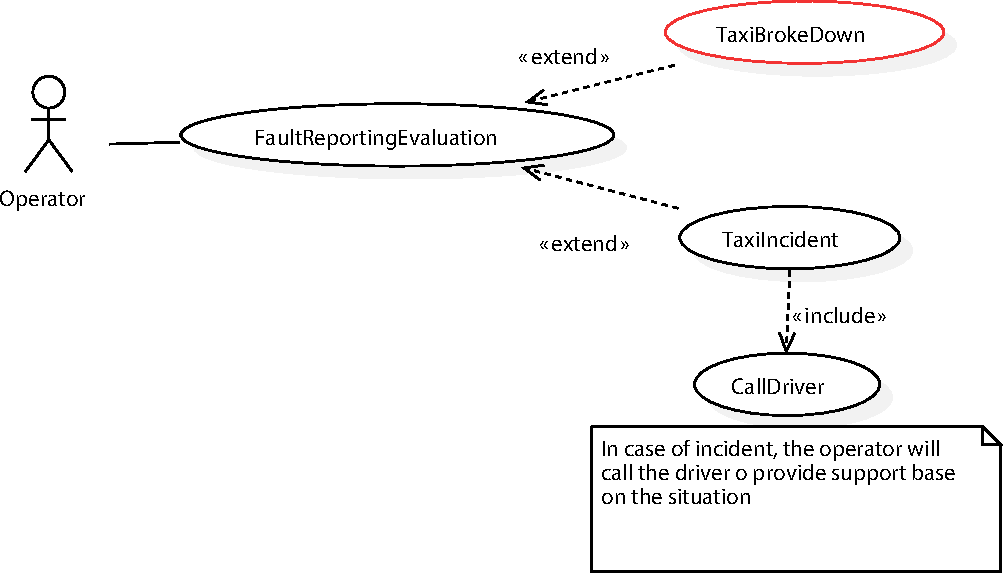
\includegraphics[width=\linewidth]{img/U_FaultReportingGLOBAL}
\end{figure*}


\begin{tabularx}{\fullwidthlength}{ l X }
	\toprule
	name				&	TaxiBrokeDown
	\\ \midrule
	actors				&	Operator
	\\ \midrule
	entry conditions	&	TaxiDriver reported a fault
	\\ \midrule
	flow of events		&	\begin{enumerate}
	
		\item the operator gets the GPS position of the taxi;
		
		\item if a customer is on board, the operator provides a new taxi, like in TaxiAllocation use case; if the taxi breaks down while reaching customer position, a new taxi is allocated directly to the customer;
		
		\item the operator calls the breakdown service.
	
	\end{enumerate} \\ \midrule
	exit conditions		&	another taxi is allocated
		\\ \midrule
	exceptions			&	\begin{itemize}
		
		\item no exception apply
	
	\end{itemize}\\ \bottomrule
\end{tabularx}


\begin{figure}
	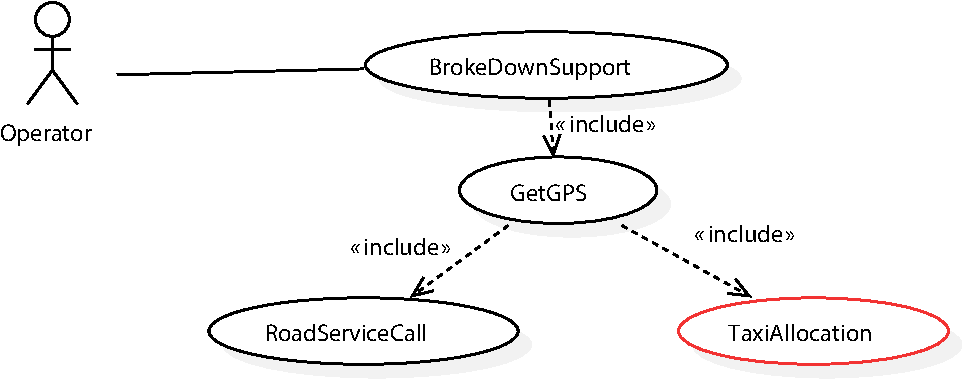
\includegraphics[width=\linewidth]{img/U_TaxiBrokeDown}
\end{figure}
	

\subsection{Taxi Available}

\paragraph{Scenario}{\small\itshape Whenever a taxi driver marks himself as ``available'' or, if already available, changes area, the system detects his new position by the on board GPS and queues him at the bottom of the queue in that specific area.}


\section{Functional requirements}
It is also useful to sum up all the functional requirements. It is important to point out that they all come as a consequence of what was stated in the previous section.


\begin{enumerate}
	\item The service shall accept only valid input: \begin{enumerate}
		\item The service shall assure that each provided address exists.
		\item The service can accept only requests with full personal data of the customer (name, surname and phone number).
	\end{enumerate}
	
	\item The service shall guarantee the non-ubiquity of the actors: \begin{enumerate}
		\item A taxi driver must be registered once.
		\item A registered customer can be registered only once.
		\item A taxi shall be registered only once.
		\item A taxi must have one and only one taxi driver, a taxi driver must have one and only one taxi.
	\end{enumerate}
	
	\item The system has to ensure the security in the login process: \begin{enumerate}
		\item Only registered customer can login in myTaxiApp.
		\item Only verified taxi driver can login in myTaxiAssist.
	\end{enumerate}
	
	\item The service shall provide a method to verify the driver: \begin{enumerate}
		\item Only authorised personnel can add or remove a taxi driver and/or a taxi.
	\end{enumerate}
	
	\item The service shall accept only valid reservations: \begin{enumerate}
		\item The service shall allow only registered customers to reserve a taxi.
		\item The system shall accept reservations only if they are made between 24 hours and 2 hours before the request time.
	\end{enumerate}
	
	\item The service shall guarantee a correct taxi allocation: \begin{enumerate}
		\item One taxi cab every four passengers must be allocated by the system.
		\item The service must ensure that a taxi is allocated to only one request at the same time.
		\item A non available taxi cab shall not be allocated to a request.
		\item The service has to provide a taxi to a customer within 10 mins.
		\item The service has to guarantee a fair management of the taxi queue.
		\item When a taxi driver refuses a request, the system must push the taxi at the end of the queue.
		\item While a taxi has a customer on board, it cannot be allocated.
		\item If a request has been accepted by the system, the customer must be taken to its destination: \begin{enumerate}
			\item If the taxi driver refuses the request, the request is forwarded to the first taxi in the queue.
			\item If no taxis are available in the area, the first taxi in the queue of adjacent areas must be selected.
			\item If the taxi breaks down, another taxi has to be allocated.
		\end{enumerate}
	\end{enumerate}
 
\end{enumerate}


To provide an overview on the structure of the system, we show here a class diagram of the whole system:


\begin{figure*}
	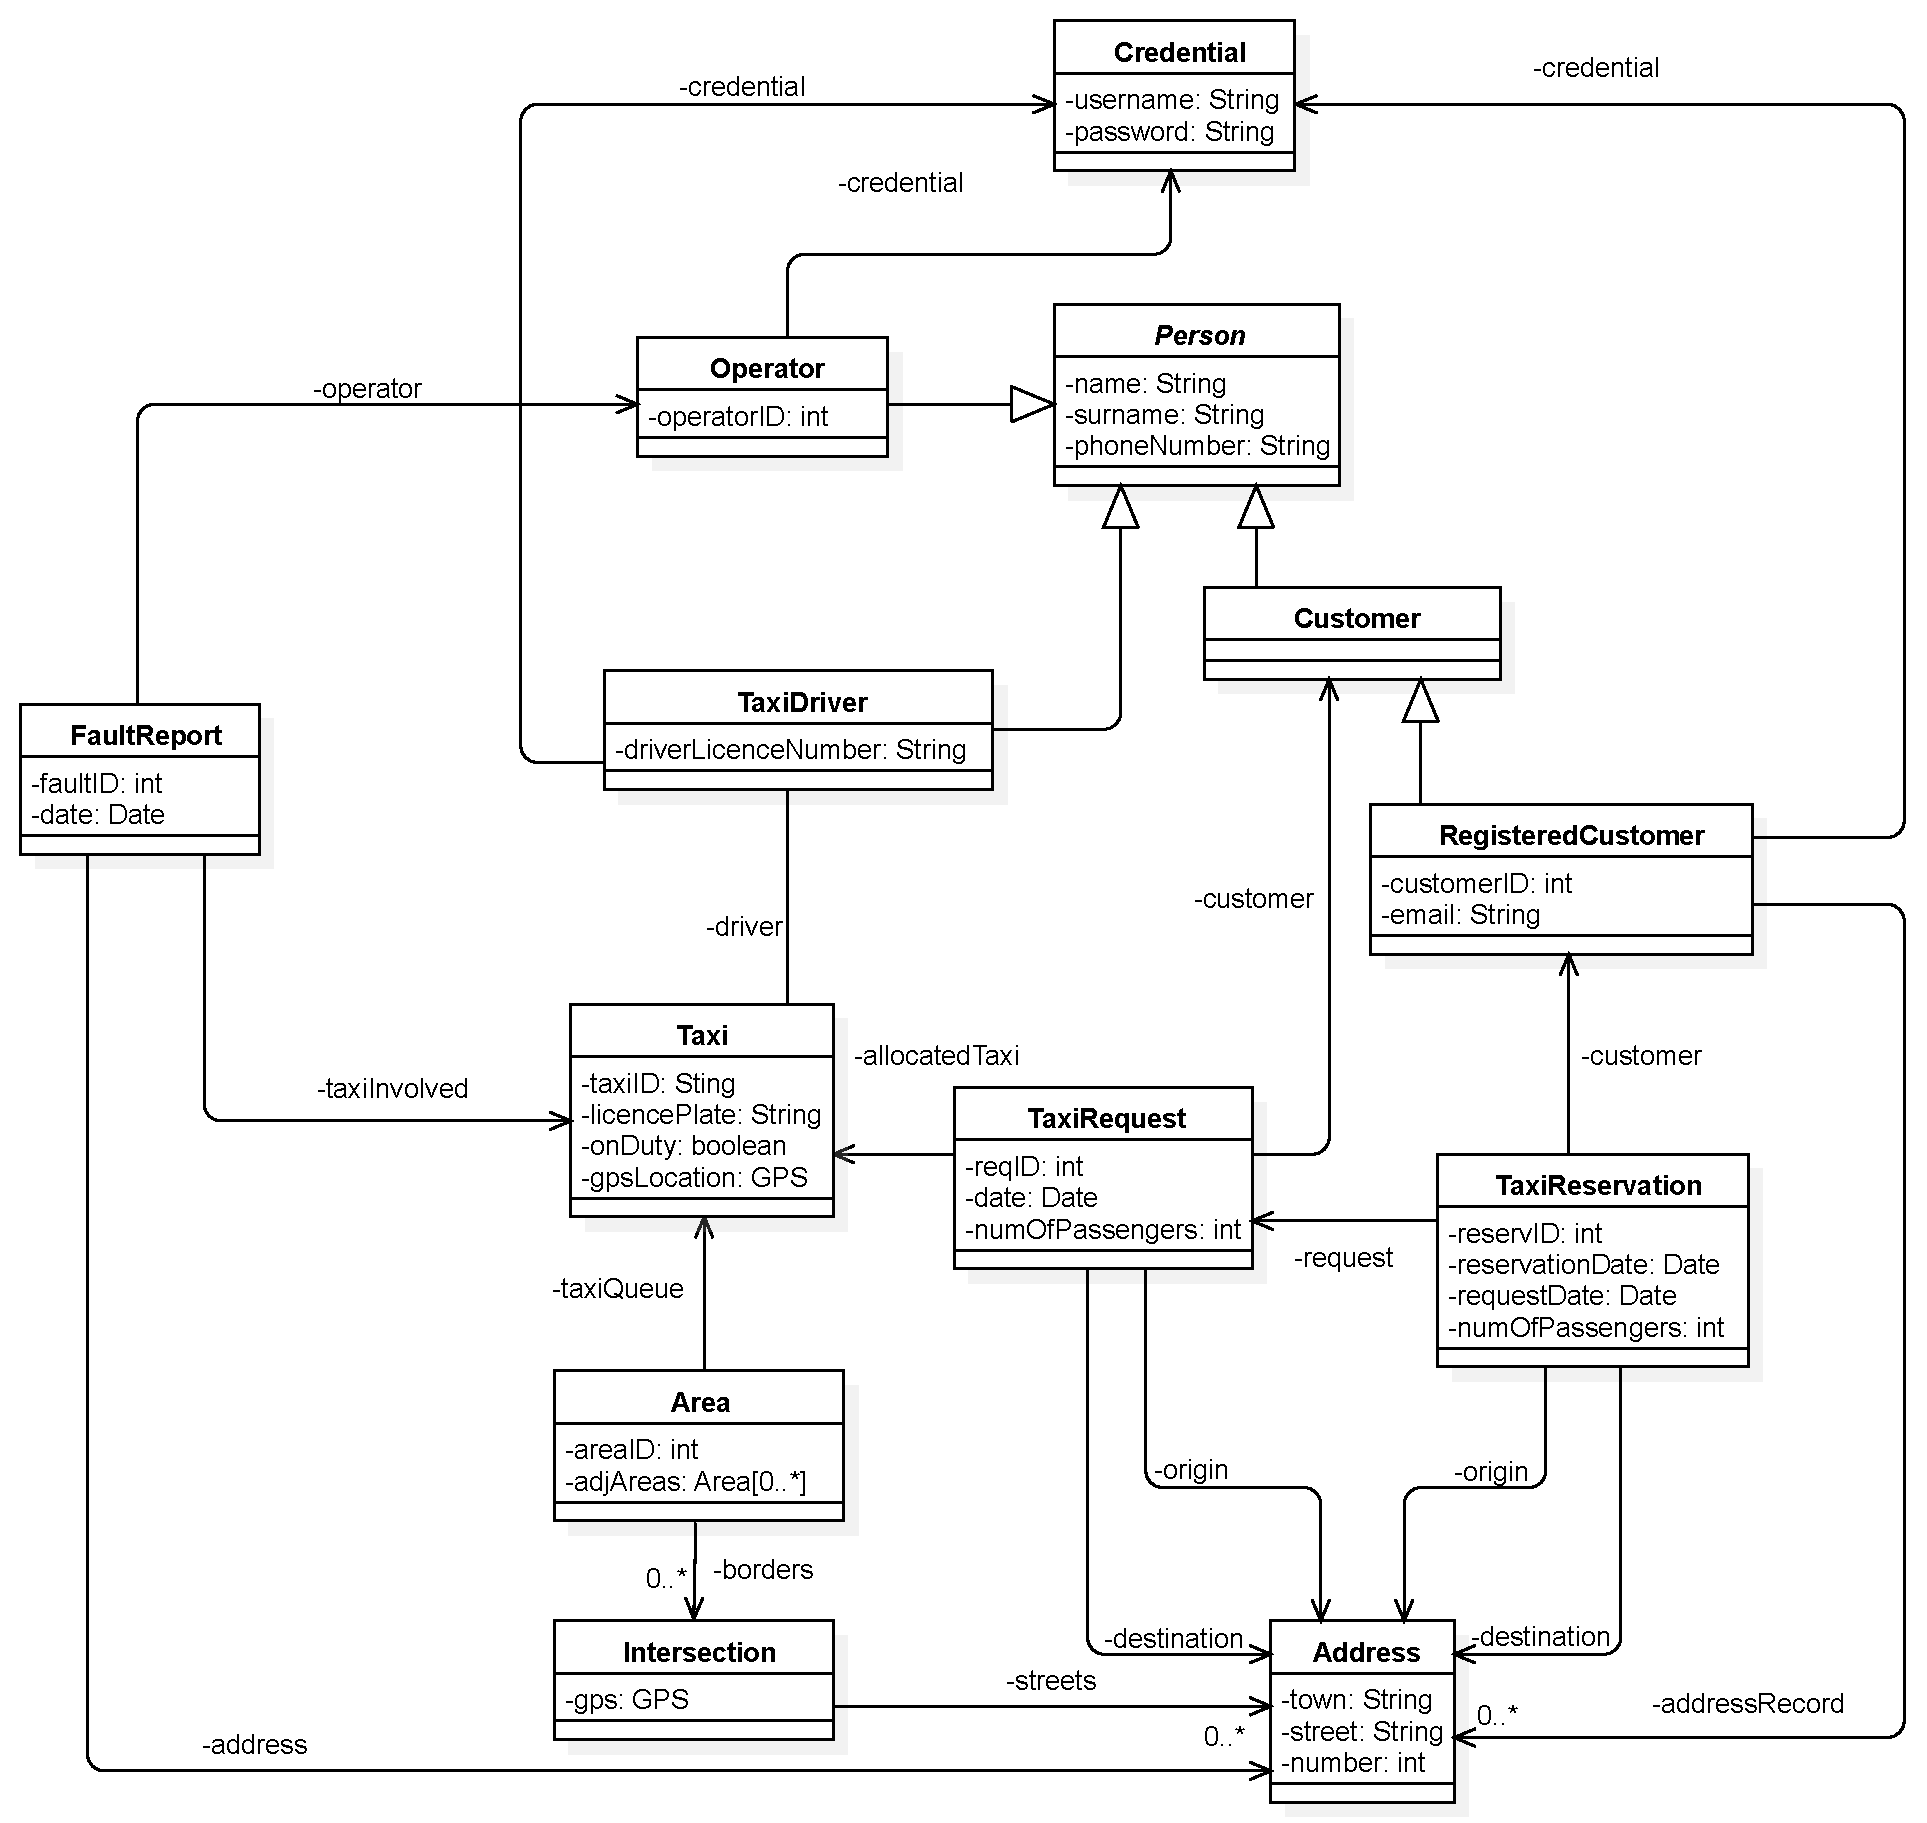
\includegraphics[width=\linewidth]{img/C_ClassDiagram.pdf}
\end{figure*}


\section{Performance requirements}
The system has to support the simultaneous connection of all taxi drivers, who are estimated to be around \num{4000}. We expect to have about \num{5} customers per taxi per hour during rush hours\footnote{This estimation was calculated by dividing the mean time to cross an area (\num{10} minutes) by one hour duration (\num{60} minutes), and then subtracting \num{1}.}, so we need to support the simultaneous connection of at least \num{20000} users, plus the users that connects to reserve a taxi for the day, that are estimated to be less numerous.

Each user exchange mainly small amounts of textual data, such as dates and addresses.

We can estimate that most users, during peak workload, are looking for a taxi in the immediate, so the system shall respond at the \SI{90}{\percent} of the requests within \num{2} seconds and a taxi should reach the customer within \num{10} minutes for the \SI{98}{\percent} of the requests. The reservation can be considered not a priority during rush hours, so the system shall respond to them within \num{5} seconds.

During normal workload, between 9AM and 4PM, we expect that most requests are going to be for reservations, which will be distributed during the day, so we expect a response time of less than \num{1} second for \SI{99,9}{\percent} of all the incoming request.


\section{Logical database requirements}
We need the database to process at least \num{6000} transactions per second.

As of the total number of registered users, there is no reasonable limit to state.


\section{Design constraints}
Actually, there is no major design constraint to take into account.


\section{Software system attributes}
There are a number of attributes of software that can serve as requirements, which we will explore in the following subsections.

\subsection{Reliability}
The system does not cover critical functions, so minor inconsistencies and faults in data integrity may be acceptable, however undesirable. The cloning method, already stated in Software interfaces subsection (\ref{subsec:systemInterfaces}), may be of help to reach this target. 

Anyway, the reliability of the system is related to the reliability of the server it runs on, so there is no point in stating strict reliability constraints.


\subsection{Availability}
We expect no more than a few hours of downtime during one year. To be more specific, we look for an availability of \SI{99,9}{\percent} of uptime, considering possible technical faults and maintenance activities. 


\subsection{Security}
All communications to and from the system shall be done over an HTTPS protocol, to guarantee the confidentiality of login credentials and personal data.

For legal purposes, a record of all taxi rides is kept. In future, it may become necessary to redefine the queue policy in area according to expected affluence, so these records have also statistic purposes.

The system shall ensure that personal data are accessible only in defined cases and for specific uses: 
\begin{itemize}
	
	\item only government can access full user's personal data;
	
	\item specific situations may require that the taxi driver calls the customer, so upon request an operator can provide customer's number to the driver; the request is registered;
	
	\item customer's personal data shall never be provided to other users;
	
	\item operators can access driver's phone number and taxi information; the access is registered.

\end{itemize}


\subsection{Maintainability}
As of the code, we want it to be well documented (namely, at least \SI{90}{\percent} of the code should be covered by comments and documentation). This will facilitate further interventions, in future. 

As best practice that should be followed in every object-oriented application (and that shall be followed for this project) is the adoption of the Model-View-Controller architectural pattern. 


\subsection{Portability}
myTaxiService has no need of portability, since it will not be a distributed system. As of myTaxiApp and myTaxiAssist, please refer to section \ref{sec:productPerspective} for every compatibility constraint.